% This is a template for BU-ECE Technical Report.
%
% Depending on report content and author preference, a BU-ECE report may be
% in one of the two following styles:
%
%   - genuine report based on ``report'' style, i.e., with chapters, much like
%     a thesis; can be single- or double-sided,
%
%   - report based on ``article'' style, i.e., with no chapters (only sections,
%     subsections, etc.), much like a journal or conference paper; can be
%     single- or double-sided.

% =====================================================================

%\documentclass[12pt]{report}          %Single-sided report style (chapters)
%\documentclass[12pt,twoside]{report}  %Double-sided report style (chapters)
%\documentclass[12pt]{article}         %Single-sided article style (no chapters)
\documentclass[12pt,twoside]{article} %Double-sided article style (no chapters)

\usepackage{bu_ece_report}
\usepackage[utf8]{inputenc}
\usepackage[spanish]{babel}
\usepackage{amsmath}
\usepackage{amsfonts}
\usepackage{amssymb}
\usepackage{makeidx}
\usepackage{graphicx}
\usepackage{lmodern}
\usepackage{float}

% In case an adjustment of vertical or horizontal margins is needed
% due to particular LaTeX/dvips or OS installation, you can uncomment
% and edit the following definitions.
% -------------------------------------------------------------------
%\topmargin       0.00 in
%\oddsidemargin   0.50 in
%\evensidemargin  0.00 in

\begin{document}

% Definitions.
% ------------
\buecedefinitions%
        {SEGUROS DE SALUD TRAS LA PANDEMIA: MEDIR LA TRANSFORMACIÓN}
        {SEGUROS DE SALUD TRAS LA PANDEMIA. INFORME 3}
        {David Moriña, Amanda Fernández-Fontelo y Montserrat Guillén}
        {Febrero 2023}
        {YYYY-NN} % Number of the report (four year digits and number)

% Box with title to fit the opening in the cover
% (adds an empty page in double-sided printing mode).
% ---------------------------------------------------
\buecereporttitleboxpage

% Title page
% (adds an empty page in double-sided printing mode).
% ---------------------------------------------------
\buecereporttitlepage

% Special page, e.g., if the report is restricted or
% to whom it is dedicated, etc., otherwise skip.
% (adds an empty page in double-sided printing mode).
% ---------------------------------------------------
%\bueceprefacepage{Here comes a special preface page. For example, if the report
%is restricted, then a suitable note can be included. This page can also be used
%to indicate to whom the document is dedicated, etc.}

% Report summary; max. 1 page.
% (adds an empty page in double-sided printing mode).
% ---------------------------------------------------
\pagenumbering{roman}
\setcounter{page}{1}
\buecereportsummary{En este tercer informe se presentan los resultados de la metodología desarrollada en el marco de este proyecto en relación al impacto de la pandemia de Covid-19 y la post-pandemia comparado con el periodo regular, tomado como referencia y definido como el periodo entre el 01-01-2019 y el 13-03-2020. En este caso puede verse que el modelo propuesto es capaz de detectar el descenso en el número de visitas al servicio de obstetricia en la provincia de Tarragona producido en el periodo de pandemia y el aumento producido posteriormente, como consecuencia de la pandemia. Adicionalmente se propone una metodología basada en series temporales Bayesianas estructurales recientemente propuesta en la literatura que puede ser útil para analizar esta cuestión desde otra aproximación y limitando los requerimientos computacionales considerablemente.} 

%LA IDEA ÉS DEDICAR AQUEST INFORME A LES ANÀLISIS DE LES DADES DE MAPFRE EXCLUSIVAMENT. DESPRÉS FALTARÀ UN INFORME GLOBAL, QUE ENTENC SERÀ LA UNIÓ/RESUM DELS ALTRES TRES.

% Table of contents, list of figures and list of tables.
% ``\bueceemptypage'' adds empty page in double-sided
% printing mode and performs ``\clearpage'' in single-sided
% mode.
% ------------------------------------------------------
\tableofcontents\bueceemptypage
\listoffigures\bueceemptypage
\listoftables\bueceemptypage

% Switch on running headers for the report:
%   odd pages  - title (lowercase); if too long, use
%                the first few words followed by ``...'',
%   even pages - last names of the authors.
% -------------------------------------------------------
\buecereportheaders

% Introduction.
% -------------
\pagenumbering{arabic}
\setcounter{page}{1}

\section{Introducción}  % Article style
Hasta 2020, el impacto de una pandemia en el seguro de salud se reconoció como un riesgo catastrófico potencial que podría afectar la frecuencia y la gravedad de las reclamaciones. Se esperaba que una pandemia aumentara el costo del seguro de salud.
Después del brote de Covid-19 en 2020, se han aprendido algunas lecciones. La pandemia ha causado una interrupción sin precedentes en el mercado mundial de seguros de salud, pero la reacción es algo diferente según el país. En los EE. UU., las compañías de seguros de salud han sufrido financieramente debido a la pandemia, y muchas reportaron pérdidas financieras, incluido el aumento de las reclamaciones y la disminución del cobro de primas. Porque la pandemia también ha provocado una disminución en el número de personas que se inscriben en planes de seguro médico. Esto se debe a la pérdida del trabajo y la reducción de los ingresos, así como a los cambios en las regulaciones de los seguros de salud. Como resultado, muchas compañías de seguros de salud se han visto obligadas a reducir los costos, incluida la reducción de la cobertura y el aumento de las primas, lo que a su vez ha provocado una disminución en la cantidad de personas que reciben cobertura de seguro de salud.
En algunos otros países, especialmente aquellos con un marcado sistema dual público-privado de salud, el efecto sobre el seguro privado de salud fue inesperado. La pandemia hizo que muchas personas se quedaran en casa, disminuyó el número de citas médicas, ingresos hospitalarios y otros servicios médicos. Esto, a su vez, condujo a una disminución en el número de siniestros asociados a los seguros de salud. La disminución de las reclamaciones también se debió a la postergación de procedimientos médicos electivos, como cirugías y otros tratamientos invasivos, que normalmente están cubiertos por los seguros de salud. Estos procedimientos a menudo se suspendieron debido a la presión sobre los sistemas de atención médica, así como a las restricciones de movimiento en muchas áreas. Como resultado, el número de reclamos relacionados con estos procedimientos disminuyó significativamente. Finalmente, el temor de contraer Covid-19 en entornos de atención médica hizo que algunas personas evitaran buscar atención médica, incluso para afecciones graves que normalmente requerirían la cobertura de un seguro médico. Esto también contribuyó a la disminución de los siniestros de seguros de salud. En general, la disminución de las reclamaciones de seguros de salud durante la pandemia se puede atribuir a una combinación de factores y también se esperaba un repunte una vez que pasara la pandemia.
Muchas aseguradoras se dieron cuenta de que 2020, 2021 y 2022 fueron años especiales en el seguro de salud y los actuarios están desconcertados por los efectos a largo plazo de los registros de siniestros. El principal problema es identificar si las fluctuaciones en la frecuencia y severidad de los siniestros vuelven a un nivel estable después de tres años, si la tarificación inmediata del seguro de salud puede resolverse descartando estos tres años, o si al menos 2022 podría tomarse como representativo para establecer tarifas en un futuro próximo. Una herramienta para corregir la información de siniestros basada en una evaluación cuantitativa del subregistro/sobredeclaración de siniestros podría ser de gran interés para basar los precios futuros en los años más recientes en lugar de recurrir a 2019 como referencia.

En este informe se presentan los resultados obtenidos mediante dos metodologías que permiten cubrir estos tres objetivos: 1) identificación de la serie temporal de puntos de ruptura de siniestros, 2) cuantificación de la magnitud del impacto de la pandemia en la frecuencia de siniestros y 3) una prueba para decidir si la serie de frecuencia de siniestros aún muestra algún impacto.

% Following sections, subsections, etc.
% -------------------------------------
\section{Métodos}
Además de la nueva metodología desarrollada en el contexto de este proyecto y descrita en los informes previos, este informe propone un enfoque basado en series temporales Bayesianas estructurales, que adapta la conocida metodología de diferencia en diferencias (\textit{difference-in-differences}) al contexto de las series de tiempo mediante el modelado explícito del contrafactual de una serie temporal observada tanto antes como después de la ocurrencia de un evento de interés, lo que podría impactar en la evolución del proceso, cómo la pandemia de Covid-19 en este caso. Este enfoque permite superar algunas de las limitaciones de la nueva metodología desarrollada, derivada del hecho de estar basada en modelos de series temporales discretas y con un coste computacional alto que resulta inasumible cuando el número de eventos analizados es demasiado grande. En las dos aproximaciones propuestas se ha usado el programa \textbf{R} (\cite{r_core_team_r_2019}), y en el caso del enfoque basado en series temporales Bayesianas estructurales se han utilizado las librerías \textit{bsts} (\cite{scott_predicting_nodate}) y \textit{CausalImpact} (\cite{brodersen_inferring_2015}). También se ha tenido en cuenta el número total mensual de contratos para controlar las tendencias observadas no relacionadas con las consecuencias de la pandemia. Para tener esta información semanalmente, se realizó un proceso de interpolación lineal usando como base la información mensual disponible.

\section{Resultados}
En esta sección se reportan los resultados de la nueva metodología desarrollada en el marco de este proyecto (subsección \textbf{Nueva metodología}) en el análisis del impacto de la pandemia de Covid-19 entre marzo y junio de 2020 y el impacto posterior en 2021 sobre el número semanal de visitas al servicio de obstetricia en la provincia de Tarragona. En todos los casos se consideran dos escenarios diferentes en cuanto a la definición del periodo post-pandemia a comparar con el periodo regular (01-01-2019 al 13-03-2020) y el periodo pandémico (14-03-2020 al 21-06-2020). El primer enfoque para la definición del periodo posterior a la pandemia (etiquetado como escenario 1 en las figuras y tablas) es comparar el periodo 01-01-2019 a 21-06-2020 contra el periodo 22-06-2020 a 31-12-2021. El segundo enfoque (etiquetado como escenario 2 en las figuras y tablas) es excluir el periodo de pandemia y comparar el periodo 01-01-2019 a 13-03-2020 contra 21-06-2020 a 31-12-2021.

\subsection{Nueva metodología}
En este apartado se describen los resultados del análisis de la comparación del periodo pandémico y post-pandémico con el periodo regular sobre el número semanal de visitas al servicio de obstetricia en la provincia de Tarragona de según la metodología basada en series temporales discretas desarrollada en el marco de este proyecto y descrita en los informes anteriores.

\begin{table}[H]\caption{Estimaciones correspondientes al periodo de confinamiento (14-03-2020 / 21-06-2020).}
    \centering
    \begin{tabular}{ cc }
        \hline
     \textbf{Parámetro} & \textbf{Estimación (IC 95\%)} \\ 
     \hline
     $\alpha$ & 0.85 (0.56; 1.14) \\
     $\lambda$ & 2.81 (-2.33; 7.95) \\
     $\omega$ & 0.80 (0.55; 1.06) \\
     $\phi_1$ & 0.025 (-0.015; 0.065) \\
     $\phi_2$ & 0.25 (0.13; 0.36) \\
     \hline
    \end{tabular}
  \end{table}

  \begin{table}[H]\caption{Estimaciones correspondientes al periodo post-pandémico (22-06-2020 / 31-12-2021).}
    \centering
    \begin{tabular}{ cc }
        \hline
     \textbf{Parámetro} & \textbf{Estimación (IC 95\%)} \\ 
     \hline
     $\alpha$ &  0 (-0.31; 0.31) \\
     $\lambda$ & 19.99 (13.92; 26.06) \\
     $\omega$ & 0.90 (0.74; 1.07) \\
     $\phi_1$ & 0.19 (-0.21; 0.58) \\
     $\phi_2$ & 0.61 (0.23; 0.99) \\
     \hline
    \end{tabular}
  \end{table}

Los resultados descritos en las tablas anteriores muestran que el modelo propuesto es capaz de detectar la disminución de las visitas producida en el periodo de confinamiento, con parámetros $\omega$ y $\phi_2$ significativamente distintos de cero, y $\phi_1 + 2 \cdot \phi_2 < 1$. Asimismo, el modelo también es capaz de detectar el aumento en el número de visitas del servicio de obstetricia en la provincia de Tarragona en el periodo post-pandémico, con parámetros $\omega$ y $\phi_2$ significativamente distintos de cero, y $\phi_1 + 2 \cdot \phi_2 > 1$. Además, en ambos periodos se observa que los parámetros $\alpha$ y $\phi_1$ no son significativamente distintos de cero, lo que sugiere que el modelo podría simplificarse y un modelo sin correlación temporal podría ser suficiente para modelar estos datos. El hecho de que los intervalos de confianza del 95\% para el parámetro $\omega$ incluyan el 1 en los dos periodos sugiere también una posible simplificación del modelo en el sentido de asumir que todas las observaciones del periodo del confinamiento presentan un uso por debajo de lo normal y todas las observaciones del periodo post-pandémico presentan un uso por encima de lo esperable según el periodo regular. 

\subsection{Series temporales Bayesianas estructurales}
El método basado en series temporales Bayesianas estructurales permite comparar la evolución observada de una serie de tiempo con la evolución estimada si el evento de interés no se hubiera producido. En este caso, en el siguiente apartado se analiza la evolución global del número semanal de actos médicos y del número semanal de visitas al servicio de obstetricia en todas las provincias. En las secciones posteriores se analizan las mismas series pero considerando solo los casos en las provincias de Madrid, Barcelona y Valencia respectivamente.

\subsubsection{Global}\label{global}
\begin{table}[H]\caption{Estimación del impacto de la pandemia y post-pandemia sobre el número semanal de actos médicos.}
    \centering  
      \begin{tabular}{ |c|c|c|c| }
          \hline
          \textbf{Escenario} & \textbf{Periodo} & \textbf{Efecto relativo (s.d.)} & \textbf{Prob. de efecto causal} \\ 
          \hline
       1 & Covid-19 & -44\% (1.8\%) & 99.99\% \\  
       1 & Post-covid & 18\% (9.4\%) & 99.32\% \\
       \hline   
       2 & Post-covid & 10\% (4.4\%) & 99.43\% \\
       \hline
      \end{tabular}
  \end{table}
  
  \begin{center}
      \begin{figure}[H]
        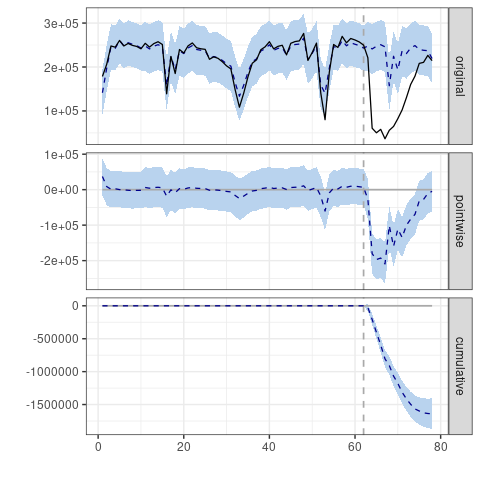
\includegraphics[width=9cm]{global_covid.png}\caption{Estimación del impacto de la pandemia sobre el número semanal de actos médicos.}
      \end{figure}\label{global_covid}
      \end{center}

Los resultados de la tabla anterior muestran una reducción significativa estimada en un 44\% del número semanal global de actos médicos en el periodo de confinamiento, y un aumento significativo en el periodo post-pandemia, tanto en la definición del escenario 1 como en el escenario 2 (que excluye del periodo post-covid el periodo de confinamiento domiciliario comprendido entre el 14-03-2020 y el 21-06-2020), estimado en el 18\% y el 10\% respectivamente.
      
  \begin{center}
  \begin{figure}[H]
    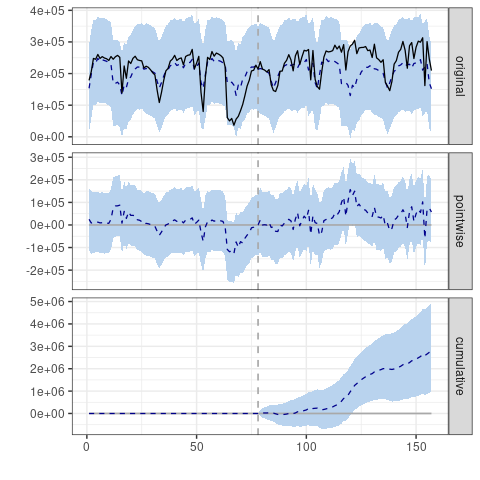
\includegraphics[width=9cm]{global_post_scen1.png}\caption{Estimación del impacto de la post-pandemia sobre el número semanal de actos médicos según el escenario 1.}\label{global_postcovid1}
  \end{figure}
  \end{center}
  
  \begin{center}
      \begin{figure}[H]
        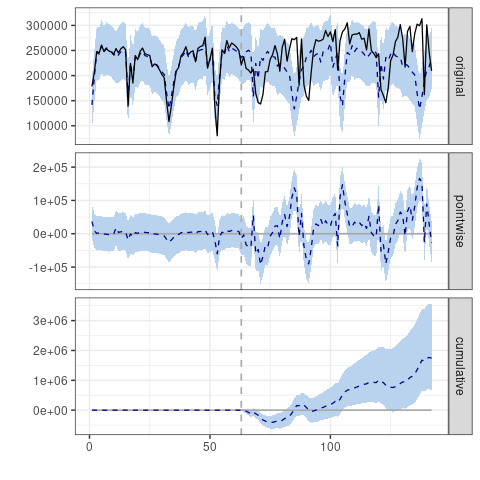
\includegraphics[width=9cm]{global_post_scen2.png}\caption{Estimación del impacto de la post-pandemia sobre el número semanal de actos médicos según el escenario 2.}\label{global_postcovid2}
      \end{figure}
      \end{center}

En las figuras~\ref{global_postcovid1} y~\ref{global_postcovid2} puede verse el aumento significativo en el periodo post-covid en cualquiera de los dos escenarios considerados.

%%%Resultats de obstetrics globalment
\begin{table}[H]\caption{Estimación del impacto de la pandemia sobre el número semanal de visitas al servicio de obstetricia.}
    \centering  
    \begin{tabular}{ |c|c|c|c| }
        \hline
        \textbf{Escenario} & \textbf{Periodo} & \textbf{Efecto relativo (s.d.)} & \textbf{Prob. de efecto causal} \\ 
        \hline
     1 & Covid-19 & -46\% (1.7\%) & 99.99\% \\  
     1 & Post-covid & 17\% (9.5\%) & 98.54\% \\
     \hline   
     2 & Post-covid & 9\% (4.3\%) & 98.52\% \\
     \hline
    \end{tabular}
  \end{table}
  
  \begin{center}
    \begin{figure}[H]
      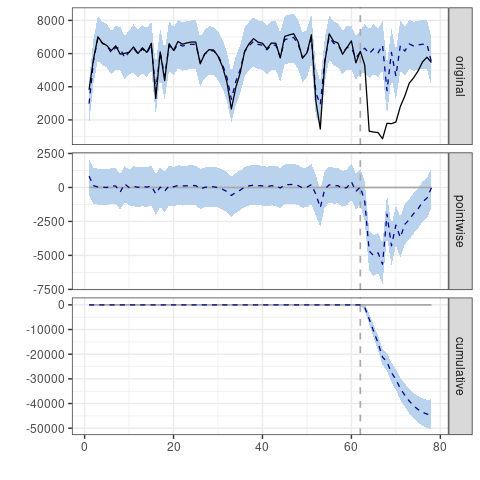
\includegraphics[width=9cm]{obstetrics_covid.png}\caption{Estimación del impacto de la pandemia sobre el número semanal de visitas al servicio de obstetricia.}
    \end{figure}
    \end{center}
    
  \begin{center}
  \begin{figure}[H]
  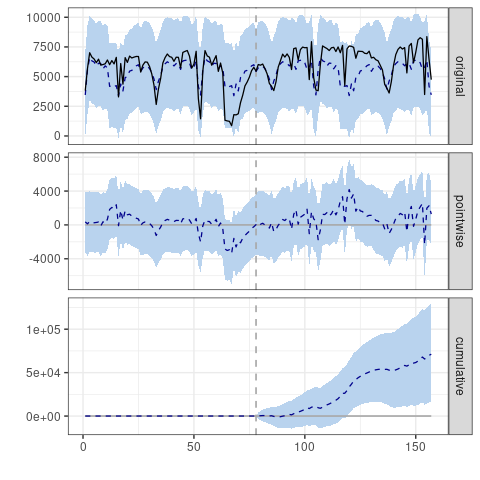
\includegraphics[width=9cm]{obstetrics_post_scen1.png}\caption{Estimación del impacto de la post-pandemia sobre el número semanal de visitas al servicio de obstetricia según el escenario 1.}
  \end{figure}
  \end{center}
  
  \begin{center}
    \begin{figure}[H]
      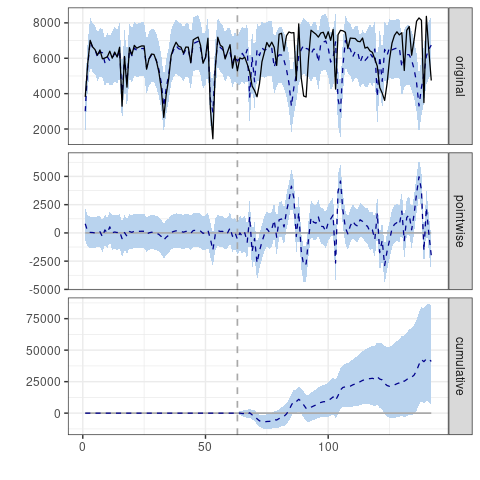
\includegraphics[width=9cm]{obstetrics_post_scen2.png}\caption{Estimación del impacto de la post-pandemia sobre el número semanal de visitas al servicio de obstetricia según el escenario 2.}
    \end{figure}
    \end{center}

De manera similar a lo descrito anteriormente, si analizamos exclusivamente la serie temporal del número semanal de visitas al servicio de obstetricia, se observa también una dismunición significativa, de alrededor del 46\% en el periodo de confinamiento domiciliario, y un aumento significativo alrededor del 17\% o del 9\% en el periodo post-covid, según los escenarios 1 y 2 respectivamente. 
    
\subsubsection{Madrid}\label{madrid}
\begin{table}[H]\caption{Estimación del impacto de la pandemia y post-pandemia sobre el número semanal de actos médicos en Madrid.}
    \centering  
      \begin{tabular}{ |c|c|c|c| }
          \hline
          \textbf{Escenario} & \textbf{Periodo} & \textbf{Efecto relativo (s.d.)} & \textbf{Prob. de efecto causal} \\ 
          \hline
       1 & Covid-19 & -48\% (1.7\%) & 99.99\% \\  
       1 & Post-covid & 9.2\% (11\%) & 92\% \\
       \hline   
       2 & Post-covid & 1.9\% (4.6\%) & 70\% \\
       \hline
      \end{tabular}
  \end{table}
  
  \begin{center}
      \begin{figure}[H]
        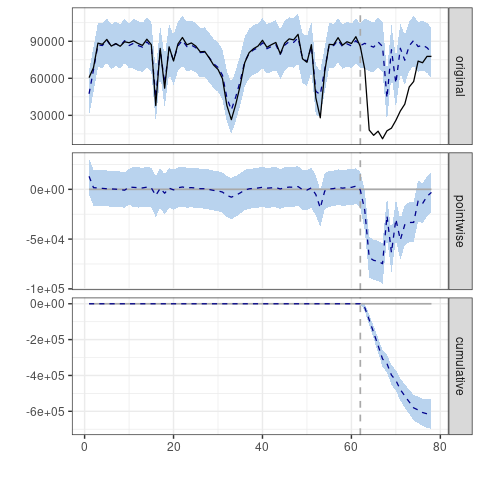
\includegraphics[width=9cm]{global_covid_Madrid.png}\caption{Estimación del impacto de la pandemia sobre el número semanal de actos médicos en Madrid.}
      \end{figure}
      \end{center}
      
  \begin{center}
  \begin{figure}[H]
    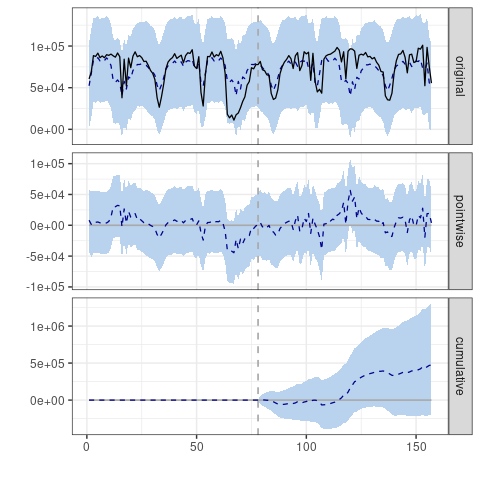
\includegraphics[width=9cm]{global_post_scen1_Madrid.png}\caption{Estimación del impacto de la post-pandemia sobre el número semanal de actos médicos según el escenario 1 en Madrid.}
  \end{figure}
  \end{center}
  
  \begin{center}
      \begin{figure}[H]
        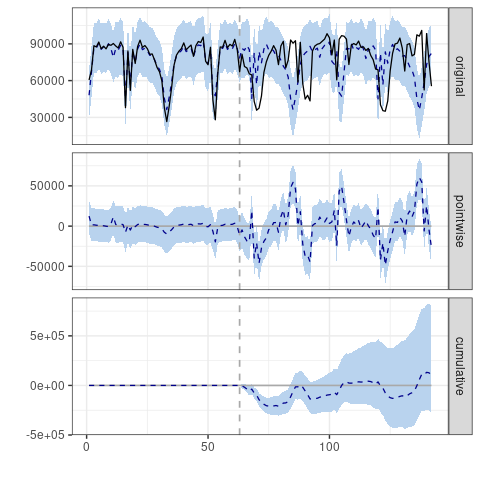
\includegraphics[width=9cm]{global_post_scen2_Madrid.png}\caption{Estimación del impacto de la post-pandemia sobre el número semanal de actos médicos según el escenario 2 en Madrid.}
      \end{figure}
      \end{center}

Los resultados muestran que en Madrid, en la línea de lo descrito en el apartado anterior, se observa una disminución significativa en el número semanal de actos médicos en el periodo de confinamiento domiciliario (estimada alrededor del 48\%), pero contrariamente a lo descrito previamente, el aumento posterior (estimado en un 9.2\% y 1.9\% para los escenarios 1 y 2 respectivamente) no resulta significativamente atribuible a las consecuencias de la pandemia.      
%%% Resultats de obstetrics a Madrid
\begin{table}[H]\caption{Estimación del impacto de la pandemia sobre el número semanal de visitas al servicio de obstetricia en Madrid.}
    \centering
      \begin{tabular}{ |c|c|c|c| }
        \hline
        \textbf{Escenario} & \textbf{Periodo} & \textbf{Efecto relativo (s.d.)} & \textbf{Prob. de efecto causal} \\ 
        \hline
     1 & Covid-19 & -51\% (1.4\%) & 99.99\% \\  
     1 & Post-covid & 11\% (9.9\%) & 94\% \\
     \hline   
     2 & Post-covid & 2.6\% (4.3\%) & 79\% \\
     \hline
    \end{tabular}
  \end{table}
  
  \begin{center}
    \begin{figure}[H]
      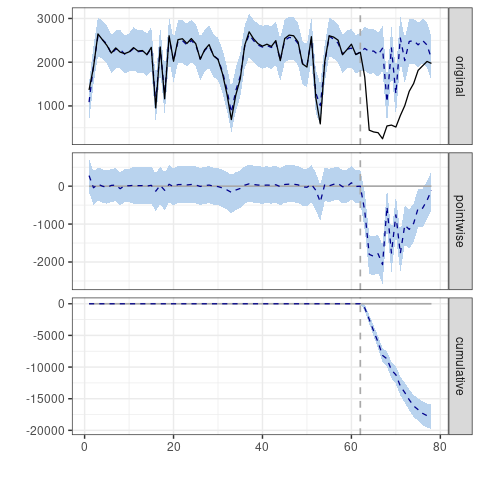
\includegraphics[width=9cm]{obstetrics_covid_Madrid.png}\caption{Estimación del impacto de la pandemia sobre el número semanal de visitas al servicio de obstetricia en Madrid.}
    \end{figure}
    \end{center}
    
  \begin{center}
  \begin{figure}[H]
  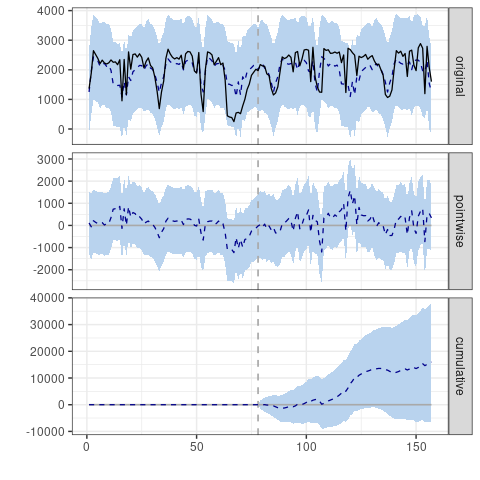
\includegraphics[width=9cm]{obstetrics_post_scen1_Madrid.png}\caption{Estimación del impacto de la post-pandemia sobre el número semanal de visitas al servicio de obstetricia según el escenario 1 en Madrid.}
  \end{figure}
  \end{center}
  
  \begin{center}
    \begin{figure}[H]
      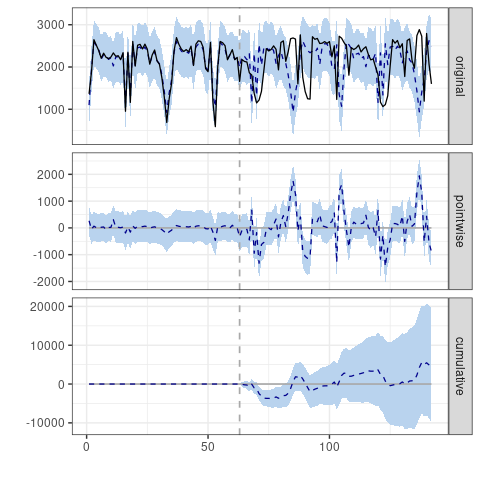
\includegraphics[width=9cm]{obstetrics_post_scen2_Madrid.png}\caption{Estimación del impacto de la post-pandemia sobre el número semanal de visitas al servicio de obstetricia según el escenario 2 en Madrid.}
    \end{figure}
    \end{center}

Respecto al análisis de la evolución del número semanal de visitas al servicio de obstetricia en la provincia de Madrid, los resultados muestran que en Madrid, en la línea de lo descrito en el apartado anterior, se observa una disminución significativa en el número semanal de actos médicos en el periodo de confinamiento domiciliario (estimada alrededor del 48\%), pero contrariamente a lo descrito previamente, el aumento posterior (estimado en un 9.2\% y 1.9\% para los escenarios 1 y 2 respectivamente) no resulta significativamente atribuible a las consecuencias de la pandemia.      

\subsubsection{Barcelona}\label{bcn}
\begin{table}[H]\caption{Estimación del impacto de la pandemia y post-pandemia sobre el número semanal de actos médicos en Barcelona.}
    \centering  
    \begin{tabular}{ |c|c|c|c| }
        \hline
        \textbf{Escenario} & \textbf{Periodo} & \textbf{Efecto relativo (s.d.)} & \textbf{Prob. de efecto causal} \\ 
        \hline
     1 & Covid-19 & -46\% (2.2\%) & 99.99\% \\  
     1 & Post-covid & 26\% (13\%) &  99.66\% \\
     \hline   
     2 & Post-covid & 16\% (4.8\%) & 99.77\% \\
     \hline
    \end{tabular}
  \end{table}
  
  \begin{center}
    \begin{figure}[H]
      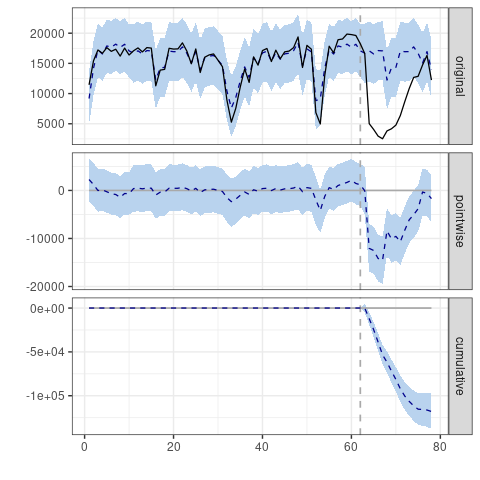
\includegraphics[width=9cm]{global_covid_Barcelona.png}\caption{Estimación del impacto de la pandemia sobre el número semanal de actos médicos en Barcelona.}
    \end{figure}
    \end{center}
    
  \begin{center}
  \begin{figure}[H]
  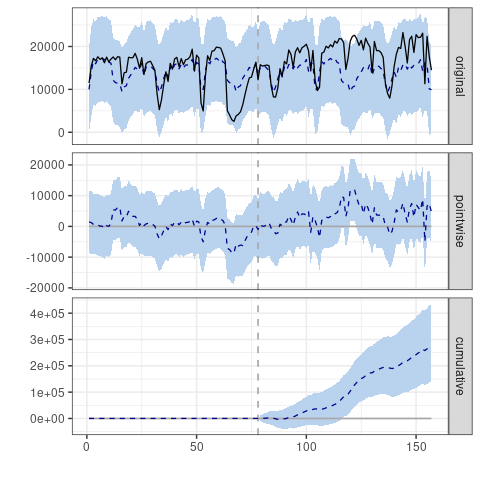
\includegraphics[width=9cm]{global_post_scen1_Barcelona.png}\caption{Estimación del impacto de la post-pandemia sobre el número semanal de actos médicos según el escenario 1 en Barcelona.}
  \end{figure}
  \end{center}
  
  \begin{center}
    \begin{figure}[H]
      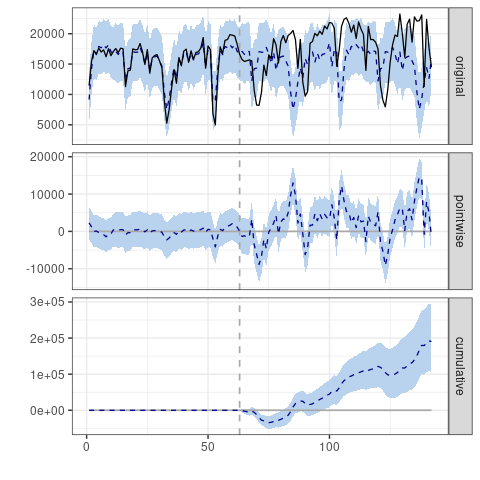
\includegraphics[width=9cm]{global_post_scen2_Barcelona.png}\caption{Estimación del impacto de la post-pandemia sobre el número semanal de actos médicos según el escenario 2 en Barcelona.}
    \end{figure}
    \end{center}

Los resultados muestran que en la provincia de Barcelona, en la línea de lo que ocurre globalmente, se observa una disminución significativa en el número semanal de actos médicos en el periodo de confinamiento domiciliario (estimada alrededor del 46\%), y el aumento posterior (estimado en un 26\% y 16\% para los escenarios 1 y 2 respectivamente) resulta también atribuible a las consecuencias de la pandemia de forma significativa.

%%% Resultats de obstetrics a Barcelona
\begin{table}[H]\caption{Estimación del impacto de la pandemia sobre el número semanal de visitas al servicio de obstetricia en Barcelona.}
    \centering  
    \begin{tabular}{ |c|c|c|c| }
        \hline
        \textbf{Escenario} & \textbf{Periodo} & \textbf{Efecto relativo (s.d.)} & \textbf{Prob. de efecto causal} \\ 
        \hline
     1 & Covid-19 & -43\% (2.3\%) & 99.99\% \\  
     1 & Post-covid & 24\% (9.2\%) & 99.53\% \\
     \hline   
     2 & Post-covid & 17\% (5\%) & 99.53\% \\
     \hline
    \end{tabular}
  \end{table}
  
  \begin{center}
    \begin{figure}[H]
      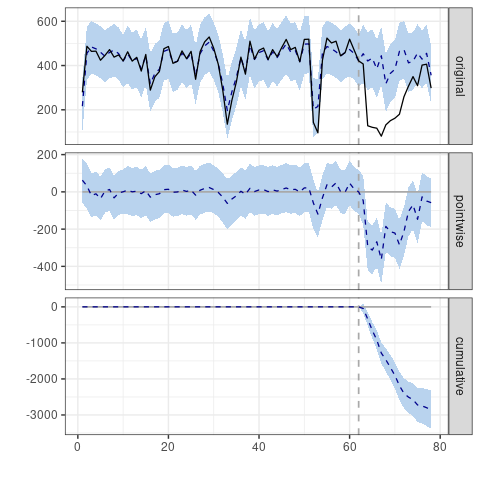
\includegraphics[width=9cm]{obstetrics_covid_Barcelona.png}\caption{Estimación del impacto de la pandemia sobre el número semanal de visitas al servicio de obstetricia en Barcelona.}
    \end{figure}
    \end{center}
    
  \begin{center}
  \begin{figure}[H]
  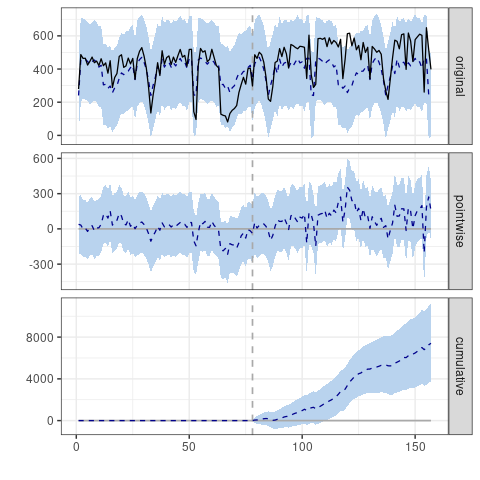
\includegraphics[width=9cm]{obstetrics_post_scen1_Barcelona.png}\caption{Estimación del impacto de la post-pandemia sobre el número semanal de visitas al servicio de obstetricia según el escenario 1 en Barcelona.}
  \end{figure}
  \end{center}
  
  \begin{center}
    \begin{figure}[H]
      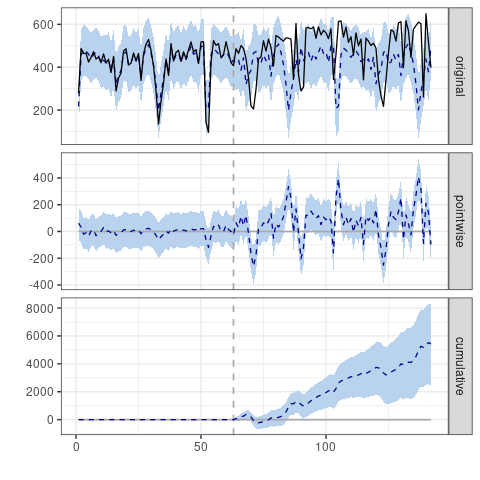
\includegraphics[width=9cm]{obstetrics_post_scen2_Barcelona.png}\caption{Estimación del impacto de la post-pandemia sobre el número semanal de visitas al servicio de obstetricia según el escenario 2 en Barcelona.}
    \end{figure}
    \end{center}

Respecto al análisis de la evolución del número semanal de visitas al servicio de obstetricia en la provincia de Barcelona, los resultados muestran que, en la línea de lo descrito anteriormente, se observa una disminución significativa en el número semanal de actos médicos en el periodo de confinamiento domiciliario (estimada alrededor del 43\%) y el aumento posterior (estimado en un 24\% y 17\% para los escenarios 1 y 2 respectivamente) resulta también atribuible a las consecuencias de la pandemia de forma significativa.      

\subsubsection{Valencia}\label{valencia}
\begin{table}[H]\caption{Estimación del impacto de la pandemia y post-pandemia sobre el número semanal de actos médicos en Valencia.}
    \centering  
    \begin{tabular}{ |c|c|c|c| }
        \hline
     \textbf{Escenario} & \textbf{Periodo} & \textbf{Efecto relativo (s.d.)} & \textbf{Prob. de efecto causal} \\ 
     \hline
     1 & Covid-19 & -41\% (2.1\%) & 99.99\% \\  
     1 & Post-covid & 28\% (10\%) &  99.83\% \\
     \hline   
     2 & Post-covid & 21\% (4.8\%) & 99.99\% \\
     \hline
    \end{tabular}
  \end{table}
  
  \begin{center}
    \begin{figure}[H]
      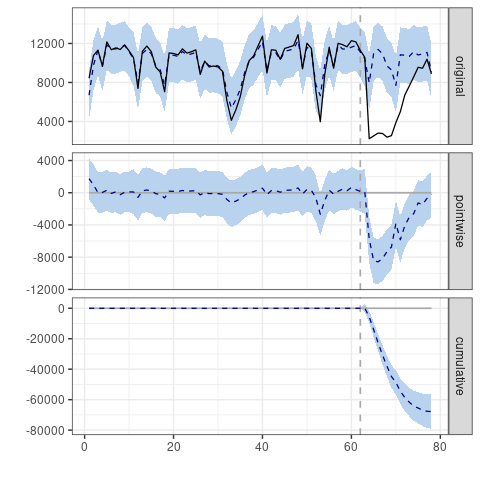
\includegraphics[width=9cm]{global_covid_Valencia.png}\caption{Estimación del impacto de la pandemia sobre el número semanal de actos médicos en Valencia.}
    \end{figure}
    \end{center}
    
  \begin{center}
  \begin{figure}[H]
  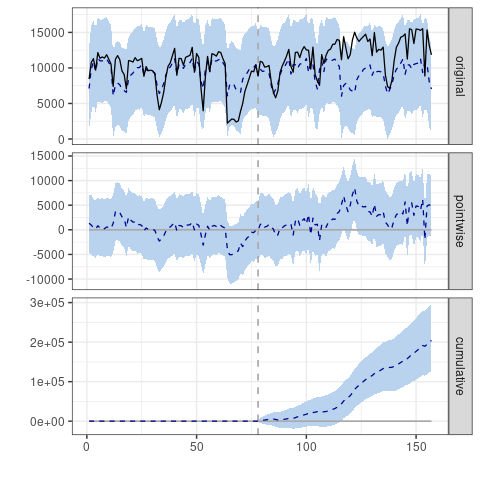
\includegraphics[width=9cm]{global_post_scen1_Valencia.png}\caption{Estimación del impacto de la post-pandemia sobre el número semanal de actos médicos según el escenario 1 en Valencia.}
  \end{figure}
  \end{center}
  
  \begin{center}
    \begin{figure}[H]
      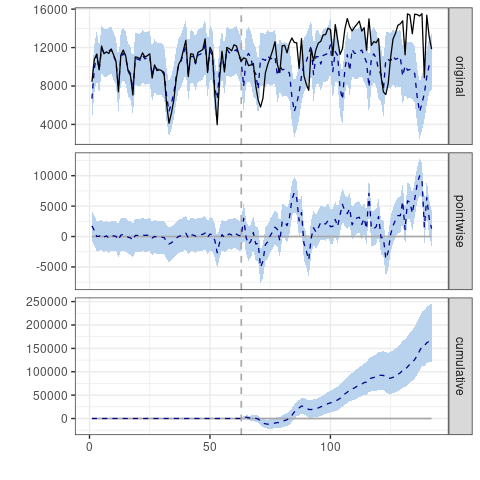
\includegraphics[width=9cm]{global_post_scen2_Valencia.png}\caption{Estimación del impacto de la post-pandemia sobre el número semanal de actos médicos según el escenario 2 en Valencia.}
    \end{figure}
    \end{center}

Los resultados muestran que en la provincia de Valencia, en la línea de lo que ocurre globalmente, se observa una disminución significativa en el número semanal de actos médicos en el periodo de confinamiento domiciliario (estimada alrededor del 41\%), y el aumento posterior (estimado en un 28\% y 21\% para los escenarios 1 y 2 respectivamente) resulta también atribuible a las consecuencias de la pandemia de forma significativa.

%%% Resultats de obstetrics a Valencia
\begin{table}[H]\caption{Estimación del impacto de la pandemia sobre el número semanal de visitas al servicio de obstetricia en Valencia.}
    \centering
      \begin{tabular}{ |c|c|c|c| }
          \hline
          \textbf{Escenario} & \textbf{Periodo} & \textbf{Efecto relativo (s.d.)} & \textbf{Prob. de efecto causal} \\ 
          \hline
       1 & Covid-19 & -42\% (2.5\%) & 99.99\% \\  
       1 & Post-covid & 32\% (9.1\%) & 99.78\% \\
       \hline   
       2 & Post-covid & 24\% (5\%) & 99.89\% \\
       \hline
      \end{tabular}
    \end{table}
    
    \begin{center}
      \begin{figure}[H]
        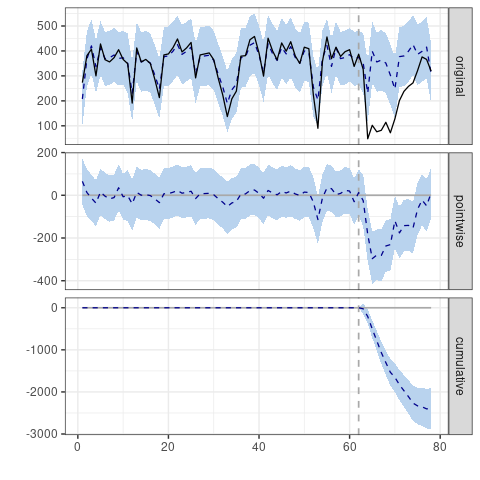
\includegraphics[width=9cm]{obstetrics_covid_Valencia.png}\caption{Estimación del impacto de la pandemia sobre el número semanal de visitas al servicio de obstetricia en Valencia.}
      \end{figure}
      \end{center}
      
    \begin{center}
    \begin{figure}[H]
    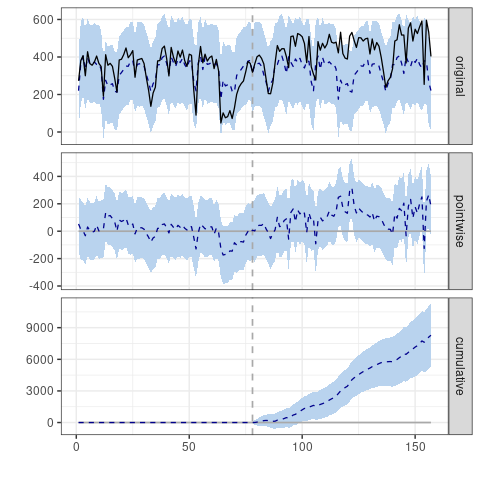
\includegraphics[width=9cm]{obstetrics_post_scen1_Valencia.png}\caption{Estimación del impacto de la post-pandemia sobre el número semanal de visitas al servicio de obstetricia según el escenario 1 en Valencia.}
    \end{figure}
    \end{center}
    
    \begin{center}
      \begin{figure}[H]
        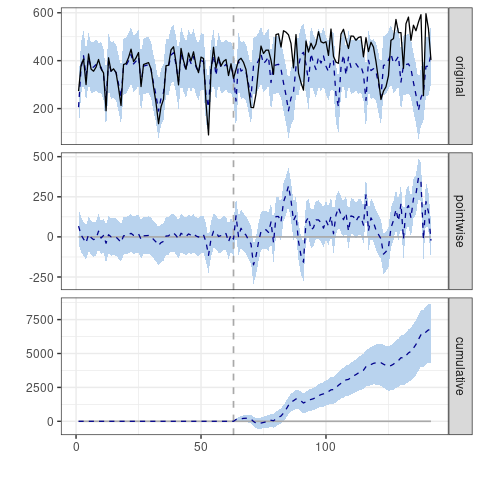
\includegraphics[width=9cm]{obstetrics_post_scen2_Valencia.png}\caption{Estimación del impacto de la post-pandemia sobre el número semanal de visitas al servicio de obstetricia según el escenario 2 en Valencia.}
      \end{figure}
      \end{center}

Respecto al análisis de la evolución del número semanal de visitas al servicio de obstetricia en la provincia de Valencia, los resultados muestran que, en la línea de lo descrito anteriormente, se observa una disminución significativa en el número semanal de actos médicos en el periodo de confinamiento domiciliario (estimada alrededor del 42\%) y el aumento posterior (estimado en un 32\% y 24\% para los escenarios 1 y 2 respectivamente) resulta también atribuible a las consecuencias de la pandemia de forma significativa.

% Bibliography.
% -------------
\parskip=0pt
\parsep=0pt
\bibliographystyle{ieeetrsrt}

% Important: substitute your BiBTeX (*.bib) files below.
% ------------------------------------------------------
\bibliography{report}

\end{document}
